\chapter{Metodología.}

\section{Calibración de la Cámara}
La calibración de la cámara es una etapa esencial para garantizar la precisión del sistema de detección de patrones y reconocimiento de formas. Este proceso se realiza utilizando técnicas estándar de calibración, como la detección de tableros de ajedrez o patrones circulares, que permiten determinar los parámetros intrínsecos y extrínsecos de la cámara. Los parámetros calculados corrigen distorsiones y aseguran una representación fiel de las figuras capturadas durante el juego.

\section{Diagrama de Bloques del Sistema}
El sistema propuesto consta de los siguientes bloques principales:
\begin{enumerate}
    \item \textbf{Calibración de Cámara:} Ajuste inicial para corregir distorsiones ópticas y asegurar imágenes precisas.
    \item \textbf{Captura de Imágenes:} Obtención de cuadros en tiempo real mediante la cámara del dispositivo.
    \item \textbf{Procesamiento de Imágenes:} Transformación de las imágenes capturadas en información útil para la detección de formas y patrones.
    \item \textbf{Reconocimiento de Formas:} Identificación de figuras geométricas basadas en las trayectorias generadas por los gestos del usuario.

    \begin{figure}[H]
    \centering
    \begin{minipage}{0.45\textwidth} 
        \centering
        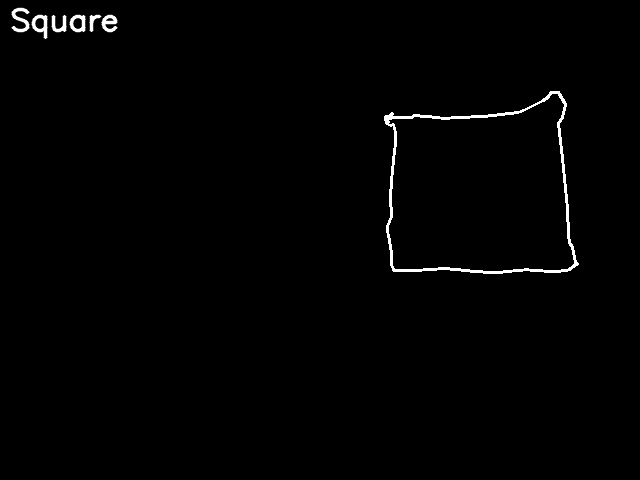
\includegraphics[width=\linewidth]{CAPS/CAP3.png}
        \caption{Detección correcta de un Cuadrado.}
        \label{fig:imagen1}
    \end{minipage}\hfill
    \begin{minipage}{0.45\textwidth} 
        \centering
        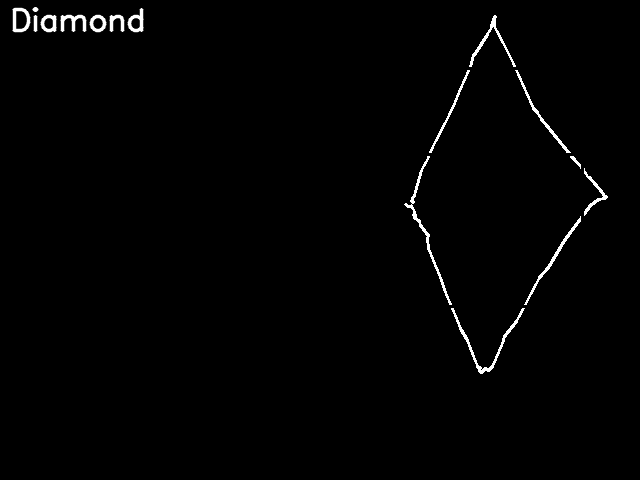
\includegraphics[width=\linewidth]{CAPS/CAP4.png}
        \caption{Detección correcta de un Rombo.}
        \label{fig:imagen2}
    \end{minipage}
    \end{figure}

    \item \textbf{Validación de Secuencias:} Comparación de las formas detectadas con las secuencias generadas para evaluar el desempeño del usuario.
    \item \textbf{Interfaz de Usuario:} Visualización en tiempo real del estado del juego y retroalimentación al jugador.
\end{enumerate}

\section{Secuencia de Transformación de Imagen}
El sistema sigue una serie de pasos para transformar las imágenes capturadas en datos procesables:
\begin{enumerate}
    \item \textbf{Captura del Frame:} Obtención de imágenes en tiempo real desde la cámara.
    \item \textbf{Conversión de Espacio de Color:} Transformación de BGR a RGB para compatibilidad con herramientas como MediaPipe.
    \item \textbf{Filtrado y Segmentación:} Aplicación de máscaras para resaltar regiones de interés, como trayectorias dibujadas.
    \item \textbf{Detección de Contornos:} Identificación de bordes y formas geométricas en las imágenes procesadas.
    \item \textbf{Reconocimiento de Figuras:} Clasificación de las figuras detectadas con base en características como el número de lados y simetría.
\end{enumerate}

\section{Sistema de Seguridad}
Para garantizar la integridad del sistema y prevenir errores en la detección, se ha implementado un mecanismo de seguridad.

\begin{figure}[H]
    \centering
    \begin{minipage}{0.45\textwidth} 
        \centering
        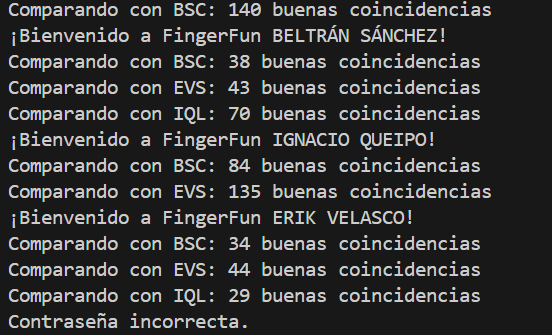
\includegraphics[width=\linewidth]{CAPS/CAP5.png}
        \caption{Detección de posibles contraseñas.}
        \label{fig:imagen1}
    \end{minipage}\hfill
    \begin{minipage}{0.45\textwidth} 
        \centering
        
\includegraphics[width=\linewidth]{CAPS/CAP6.png}
        \caption{Contraseña ejemplo.}
        \label{fig:imagen2}
    \end{minipage}
\end{figure}

\subsection{Detección de Contraseñas}
Se utiliza un modelo de detección de contraseñas en el cual se tiene una base de datos donde se guardan las contraseñas válidas. El usuario intenta desbloquear de forma intuitiva el juego mostrando dicha contraseña a la cámara, la cual reconoce los patrones y deniega accesos no deseados. 

\section{Diagrama de Bloques:}

\begin{figure}[H]
    \centering
    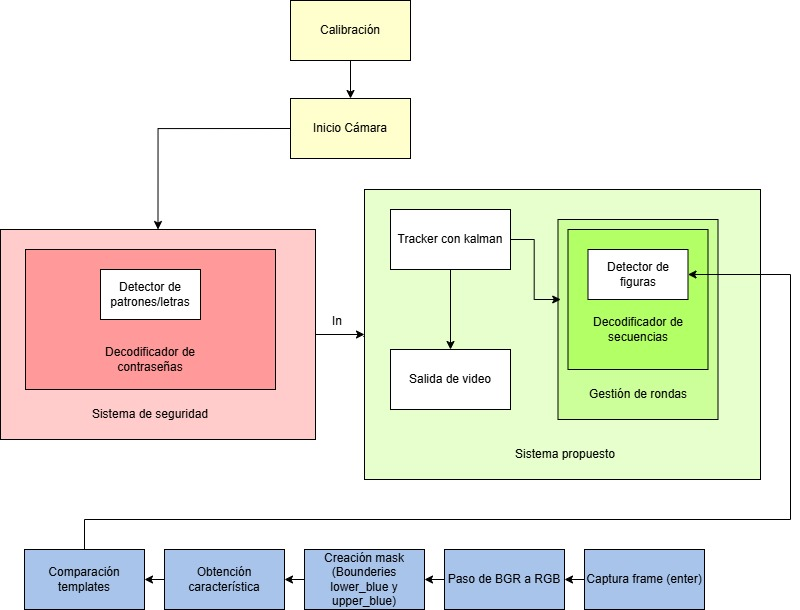
\includegraphics[width=\textwidth -2cm]{CAPS/CAP7.jpg}
    \caption{Resumen de los módulos de software.}
    \label{fig:imagenes}
\end{figure}
